
\usetikzlibrary{shapes,arrows}
\pagestyle{empty}

\chapter{Research Plan} \label{plan}

\section{Introduction}

The solutions discussed so far all have one thing in common. They provide very specific and satisfactorily accurate partial solution to the overarching process. But the complete automated feature extraction and analysis is not yet available. This work deals with a very specific standard of map where accuracy of both shape and scale are of paramount importance. All process should be completely automated for maximum efficiency. Moreover, none of these previous works deal with specific plot segmentation over a large constellation of closely arranged contours.

In this chapter we will describe problem formulation, our work plan, what we have already done and what have to be done in future. 

\section{Overview of the Problem}

A scanned paper Mouza map is taken as any available image format, such as : .png, .jpg, .bmp etc. Initially the scanned image will contain various distortions. But, after processing, the plot lines or remaining segments must form a single connected component ${C}$. Suppose after the contour analysis and template matching processes, the number of extracted number groupings are ${N}$. The image should be processed in such a way that the number of extracted plots ${n}$ match exactly with ${N}$. For that, some of the numbers that lie outside the connected component ${C}$ , equals ${r}$ must be subtracted from original numbered groups ${N}$. Transformations must be applied to obtain plot contours,
\begin{equation}
n=N-r, where r=C'
\end{equation}


\section{Work Plan}\label{todo}

We have divided our work to several steps. They are described below : 

\begin{enumerate}
    \item Removing background noise\ref{noise}
    \item Connecting broken contours\ref{closing}
    \item Contour size analysis\ref{segcon}
    \item Number detection\ref{template}
    \item Number segmentation\ref{remove}
    \item Plot contour extraction\ref{plot}
    \item Combining all the extracted subplots to make the whole mouza map\ref{merge}
\end{enumerate}


\section{Works Done So Far}

The steps \ref{noise}, \ref{segcon}, \ref{remove} and \ref{plot} described in section \ref{todo} are completed. They will be described elaborately in the following subsections.

\subsection{Noise Reduction}
Gaussian and Median filters are applied in succession. This reduces the amount of background noise. There are several specific kinds of noise prevalent in a scanned mouza map. They are mentioned below:
\begin{enumerate}
    \item Detecting moving objects in each frame
    \item Associating the detection corresponding to the same object over time
\end{enumerate}

The detection of moving objects uses a background subtraction algorithm based on Gaussian mixture models.~\cite{DBLP:conf/cvpr/StaufferG99} Morphological operations are applied to the resulting foreground mask to eliminate noise. Finally, blob analysis detects groups of connected pixels, which are likely to correspond to moving objects.

The association of detection to the same object is based solely on motion. The motion of each track is estimated by a Kalman filter. The filter is used to predict the track's location in each frame, and determine the likelihood of each detection being assigned to each track.

Track maintenance becomes an important aspect of this procedure. In any given frame, some detections may be assigned to tracks, while other detections and tracks may remain unassigned. The assigned tracks are updated using the corresponding detections. The unassigned tracks are marked invisible. An unassigned detection begins a new track.

Each track keeps count of the number of consecutive frames, where it remained unassigned. If the count exceeds a specified threshold, the example assumes that the object left the field of view and it deletes the track.

``\Cref{fig:moving} is the flowchart of tracking moving objects in a video frame.''



A short description of the total procedure is given below :

\begin{figure}[H]
  \centering
  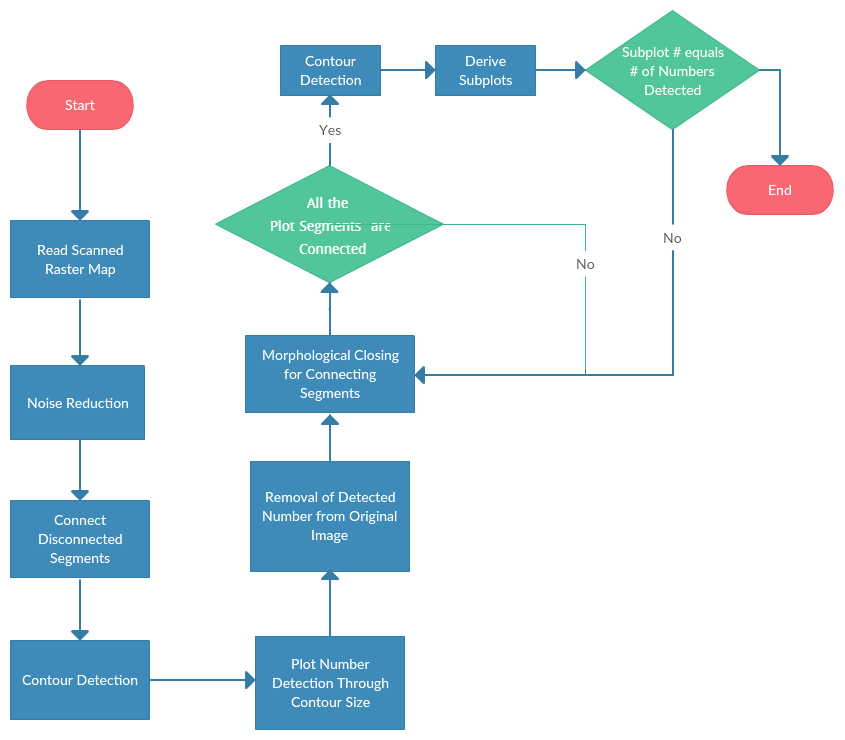
\includegraphics[width=0.9\textwidth]{figures/raster}
  \caption{Flowchart}
  \label{fig:raster}
\end{figure} 

\begin{enumerate}

    \item \textbf{Create System Object} : This is used for reading the video frames, detecting foreground objects, and displaying results. 
    
    \item \textbf{Initialize Tracks} : This creates an array of tracks, where each track is a structure representing a moving object in the video. The purpose of the structure is to maintain the state of a tracked object. The state consists of information used for detection to track assignment, track termination, and display. 
    
    \item \textbf{Read Frame} : This reads the next video frame from the video file. 
    
    \item \textbf{ Detect Objects} : The function returns the centroids and the bounding boxes of the detected objects. It also returns the binary mask, which has the same size as the input frame. Pixels with a value of 1 correspond to the foreground, and pixels with a value of 0 correspond to the background. The function performs motion segmentation using the foreground detector.~\cite{DBLP:conf/cvpr/StaufferG99} It then performs morphological operations on the resulting binary mask to remove noisy pixels and to fill the holes in the remaining blobs.
    
    \item \textbf{Predict New Locations of Existing Tracks}: This uses the Kalman filter to predict the centroid of each track in the current frame, and update its bounding box accordingly.
    
    \item \textbf{Assign Detections to Tracks} : This assigns object detections in the current frame to existing tracks is done by minimizing cost. ~\cite{Miller97optimizingmurty's,doi:10.1137/0105003}
    
    \item \textbf{Update Assigned Tracks} : The procedure updates each assigned track with the corresponding detection.
    
    \item \textbf{Update Unassigned Tracks} : This marks each unassigned track as invisible, and increases its age by 1.
    
    \item \textbf{Delete Lost Tracks} : This deletes tracks that have been invisible for too many consecutive frames. It also deletes recently created tracks that have been invisible for too many frames overall.
    
    \item \textbf{Create New Tracks} : This creates new tracks from unassigned detections assuming that any unassigned detection is a start of a new track.
    
    \item \textbf{Display Tracking Results} : This draws a bounding box and label ID for each track on the video frame and the foreground mask. It then displays the frame and the mask in their respective video players.
    
    \item \textbf{Are More Frames Available} : This checks if more video frame is available in the video clip. If it is yes, then it goes to read frame procedure and continues. If it is no then , stop the process. 
    
    
    
\end{enumerate}
   
\subsubsection{Experimental Results}
    
    We have done our experiment and simulation in MATLAB. In appendix \ref{ch:codes} at section \ref{trackcode} contains the code of tracking moving object in a video. ``Figure ~\ref{fig:car1}-~\ref{fig:man3} shows our experimental result of tracking moving objects with a boundary box in a video frame.''.

\begin{figure}[H]
  \centering
  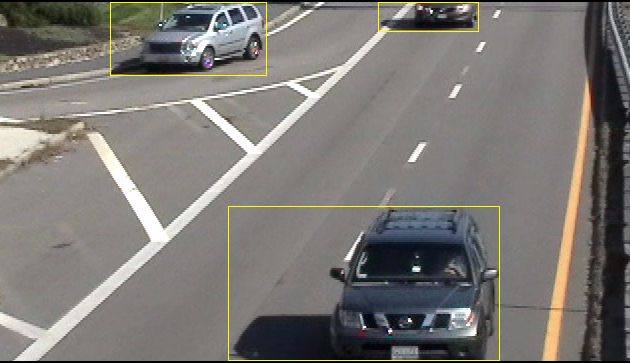
\includegraphics[width=0.9\textwidth]{figures/car1}
  \caption{Tracking Moving Objects Result.}
  \label{fig:car1}
\end{figure} 

\begin{figure}[H]
  \centering
  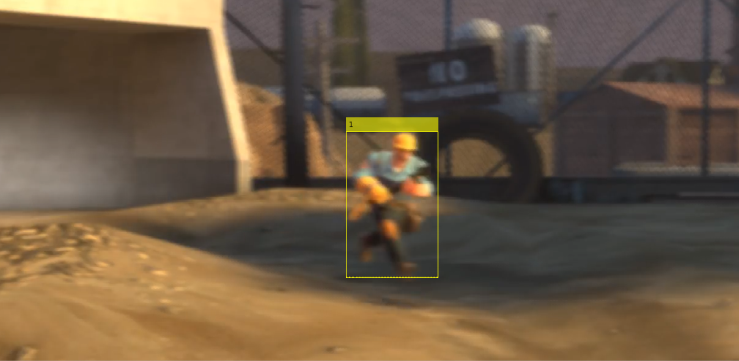
\includegraphics[width=0.9\textwidth]{figures/man1}
  \caption{Tracking Moving Objects Result.}
  \label{fig:man1}
\end{figure} 

\begin{figure}[H]
  \centering
  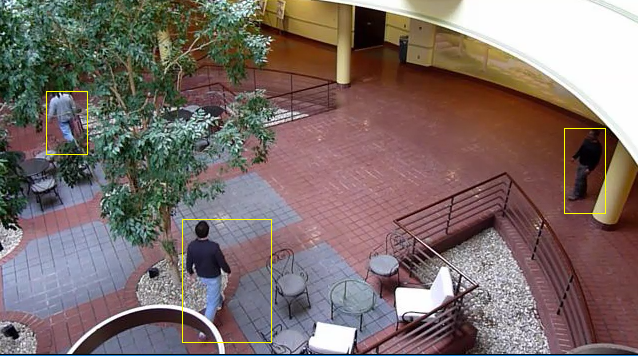
\includegraphics[width=0.9\textwidth]{figures/man3}
  \caption{Tracking Moving Objects Result.}
  \label{fig:man3}
\end{figure} 
    
Our experiment which is done in MATLAB shows good result of tracking moving objects with a boundary box in video frames.

\subsection{Tracking Velocity of Each Moving Object}\label{velocity}

After tracking moving objects, we have tracked velocity of each object . We've a boundary box associated with each object which have a centroid. In every frame, we have calculated the displacement of the centroid from the previous frame of the object. This value is velocity in  pixel per frame for that object. Multiplying it with frame rate, we got the instantaneous velocity for that frame for the object. After all the frame is explored, we divide the total displacement of that object in the video by the numbers of time the objects have appeared in all the video frames. This is the average velocity of the object in that video. The average velocity is needed when we want to predict an object's future movement. If frame rate r, total displacement in the video of a object $t_d$, number of the frames the object appears in the video n then , 
\newline
\newline
\centerline{displacement in X axis in pixel, x = centroidX - centroidX of previous frame}
\centerline{displacement in Y axis in pixel, y = centroidY - centroidY of previous frame}
\centerline{displacement in a frame in pixel, d = $\sqrt{x^2 + y^2}$}
\centerline{instantaneous velocity in pixel per second, v = d $\times r$}
\centerline{
total average velocity in the video, $v_{avg}$ = $\frac {t_d}{n}$
}

\subsubsection{Experimental Results}
    
In appendix \ref{ch:codes} at section \ref{trackcode} contains the code of tracking moving object with object id and velocity in a video.``Figure ~\ref{fig:car1v}-~\ref{fig:man3v} shows our experimental result of tracking moving objects with a boundary box in a video frame with object id and instantaneous velocity in pixel per second unit.''.

\begin{figure}[H]
  \centering
  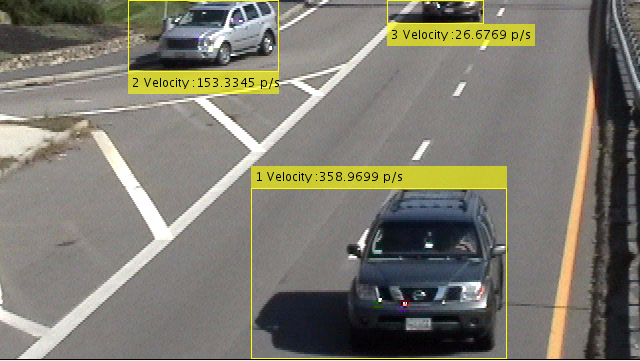
\includegraphics[width=0.9\textwidth]{figures/car1v}
  \caption{Tracking Moving Objects with Velocity in Pixel Per Second.}
  \label{fig:car1v}
\end{figure} 

\begin{figure}[H]
  \centering
  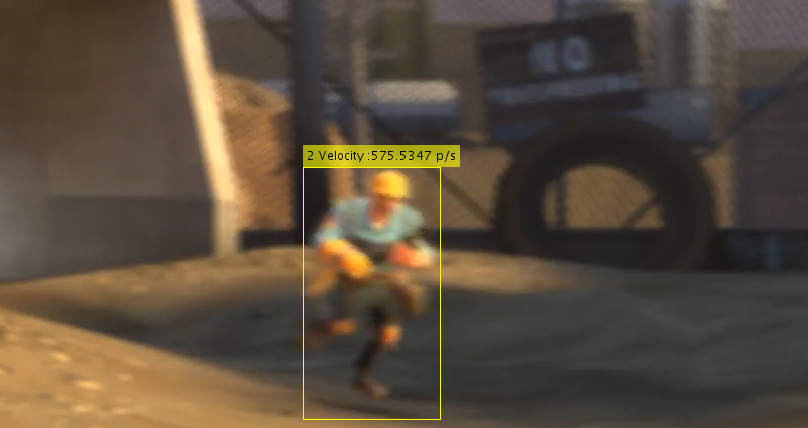
\includegraphics[width=0.9\textwidth]{figures/man1v}
  \caption{Tracking Moving Objects with Velocity in Pixel Per Second.}
  \label{fig:man1v}
\end{figure} 

\begin{figure}[H]
  \centering
  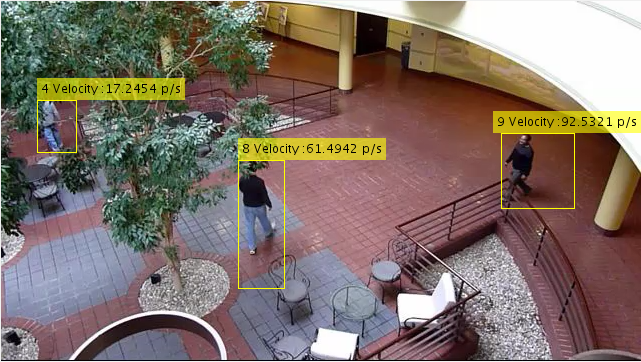
\includegraphics[width=0.9\textwidth]{figures/man3v}
  \caption{Tracking Moving Objects with Velocity in Pixel Per Second.}
  \label{fig:man3v}
\end{figure} 

\subsection{Determining Approximate Time through Prediction}

We need to predict how much time is needed by an object to pass an area where a camera is not available or the camera of the area is damaged. We can predict the time by its previous or future camera's average velocity. We've already got the average velocity described in section \ref{velocity}. Now we need a background image where a camera is not available or the camera is damaged. We also have to specify the path where the object might have passed. If we divide the total distance of the specified path by the average previous or future velocity, we will get an approximate time to pass the path for that object. If total distance is d and average velocity is $v_avg$ then,
\newline
\newline
\centerline{total approximate time, $t$ = $\frac{d}{v_{avg}}$}

\subsubsection{Experimental Results}
In appendix \ref{ch:codes} at section \ref{prediction} contains the code of determining approximate time given the object average velocity and the specified path in the background image of the area where there is no camera or the camera is damaged. ``\Cref{fig:background} shows a background image with specified path where camera not available.''.

\begin{figure}[H]
  \centering
  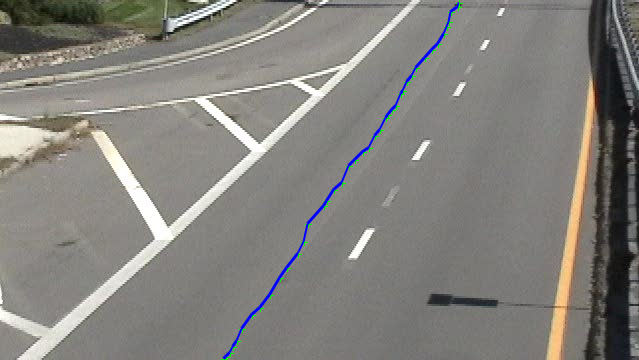
\includegraphics[width=0.9\textwidth]{figures/background}
  \caption{Background Image with Specified Path Where Camera Not Available.}
  \label{fig:background}
\end{figure} 

\endinput
